\documentclass[a4paper,12pt]{article}

\usepackage{fancyhdr}
\pagestyle{fancy}
\fancyhf{}
\rhead{Dominic Moylett - dm1905@my.bristol.ac.uk}
\cfoot{Page \thepage}

\usepackage{tikz}

\usepackage{amsmath}

\begin{document}
    \begin{center}
        \section*{Fault Tolerant Computation and VLSI Testing}
        \subsection*{Assignment 2}
    \end{center}

    \begin{enumerate}

        \item
            \begin{enumerate}
                \item $R_{BC}(t) = 1 - (1 - R(t))^2 = 2R(t) - R(t)^2$

                    $R_{ABC}(t) = R_A(t)R_{BC}(t) = 2R(t)^2 - R(t)^3$

                    $R_{ABCD}(t) = 1 - (1 - R_{ABC}(t))(1 - R_D(t))$

                    $= 1 - (R(t)^3 - 2R(t)^2 + 1)(1 - R(t))$

                    $= R(t)^4 - 3R(t)^3 + 2R(t)^2 + R(t)$

                    $R_{system}(t) = R_{ABCD}(t)R_E(t) = R(t)^5 - 3R(t)^4 + 2R(t)^3 + R(t)^2$

                \item If the life time of each of the five modules is exponentially distributed with parameter $\lambda$, then the reliability of each module is $R(t) = e^{-\lambda t}$:

                    $R_{system}(t) = e^{-5\lambda t} - 3e^{-4\lambda t} + 2e^{-3\lambda t} + e^{-2\lambda t}$
            \end{enumerate}

        \item 
            \begin{enumerate}
                \item NMR with spare means that the system will always act as an NMR system, but if any of the modules develops a fault that is detected, that module will be swapped out for a spare.

                    In the case of our example will five modules, three of the modules will be in use and the other two will act as spares. If one of the three active modules develops a fault, this is swapped out for a spare and there will be three active modules again, but only one spare left. When a second module develops a fault, this is again swapped out for the remaining spare. We are now out of spares, so the system continues as a traditional NMR (in this case TMR).

                    Self-purging redundancy has every module that hasn't yet developed a fault active at the same time. If a module develops a fault, that module is removed and the system continue with the remaining modules.

                    In the case of our five module system, the system starts off in a 5MR setup. When a module develops a fault, this module is removed and the system switches to a setup with four voting modules. When another module develops a fault, that module is also removed, leaving three voters. The system now continues as a traditional TMR.

                \item Consider the reliability diagram of the system without module C:

                    \begin{center}
                        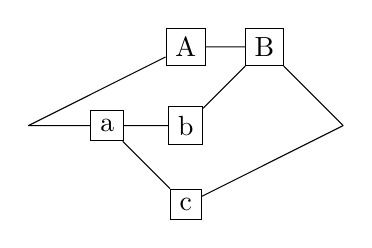
\begin{tikzpicture}
                            \tikzset{module/.style={draw, shape=rectangle}}
                            \node[module] (a) at (1, 1){a};
                            \node[module] (b) at (2, 1){b};
                            \node[module] (c) at (2, 0){c};
                            \node[module] (A) at (2, 2){A};
                            \node[module] (B) at (3, 2){B};

                            \draw (0, 1) -- (a)
                                (0, 1) -- (A)
                                (A) -- (B)
                                (a) -- (b)
                                (a) -- (c)
                                (b) -- (B)
                                (B) -- (4, 1)
                                (c) -- (4, 1);
                        \end{tikzpicture}
                    \end{center}

                    The minimum requirements for these modules to fail and the probabilities of them happening are:
                    \begin{itemize}
                        \item a and A fail - $(1 - R)^2$
                        \item a and B fail - $(1 - R)^2$
                        \item B and c fail - $(1 - R)^2$
                    \end{itemize}
                    The probability of these modules failing is therefore $3(1 - R)^2$, so the reliability for these modules is:

                    $R_{abcAB} = 1 - 3(1 - R)^2$

                    We can incorporate this into the overall system reliability as module C runs in parallel to all of these modules.

                    $R_{system} = 1 - (1 - R_{abcAB})(1 - R_C) = 1 - 3(1 - R)^3$

            \end{enumerate}

        \item
            \begin{itemize}
                \item 3S is all three modules working and the spare not in use.
                \item 3 is three modules working and the spare has either been put in for another module or has failed.
                \item 2 is two modules working and the spare has either been put in for another module or has failed.
                \item 2S is where one of the modules has failed, but the failure hasn't been detected.
                \item F is the failure state; either two modules have failed but neither were successfully detected and swapped for the spare, or three modules have failed and one was replaced with the spare.
            \end{itemize}

            \begin{center}
                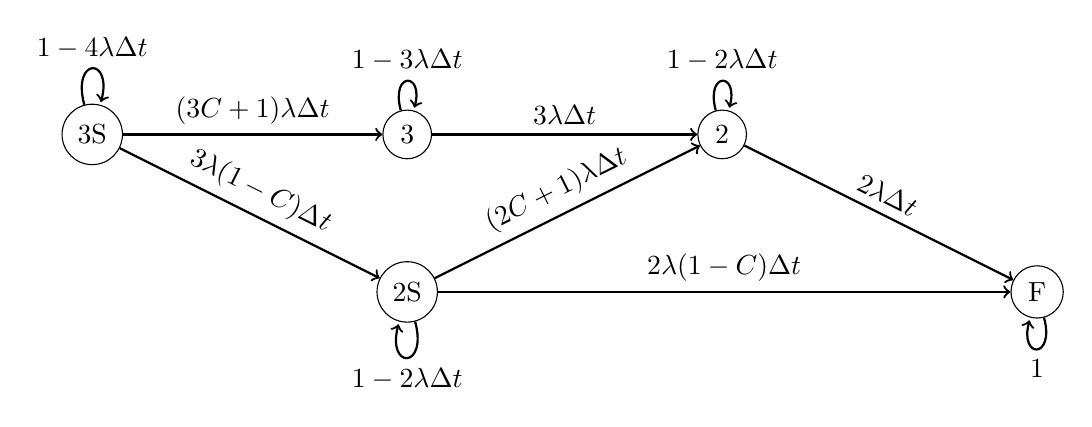
\begin{tikzpicture}
                    \tikzset{state/.style={draw, shape=circle}}
                    \node[state] (3S) at (0, 2) {3S};
                    \node[state] (3) at (4, 2) {3};
                    \node[state] (2) at (8, 2) {2};
                    \node[state] (2S) at (4, 0) {2S};
                    \node[state] (F) at (12, 0) {F};

                    \path[->, thick]
                        (3S) edge [loop above] node {$1 - 4\lambda\Delta t$} (3S)
                            edge node [above] {$(3C + 1)\lambda\Delta t$} (3)
                            edge node [above, sloped] {$3\lambda(1 - C)\Delta t$} (2S)
                        (3) edge [loop above] node {$1 - 3\lambda\Delta t$} (3)
                            edge node [above] {$3\lambda\Delta t$} (2)
                        (2) edge [loop above] node {$1 - 2\lambda\Delta t$} (2)
                            edge node [above, sloped] {$2\lambda\Delta t$} (F)
                        (2S) edge [loop below] node {$1 - 2\lambda\Delta t$} (2S)
                            edge node [above, sloped] {$(2C + 1)\lambda\Delta t$} (2)
                            edge node [above] {$2\lambda(1 - C)\Delta t$} (F)
                        (F) edge [loop below] node {$1$} (F);
                \end{tikzpicture}
            \end{center}

        \item
            \begin{description}
                \item[(1)]
                    \begin{itemize}
                        \item State 2 is where both modules are working.
                        \item State 1 is where one module has discovered a fault: Either a fault has occured in the active module and it has been discovered and swapped successfully, or a fault has occured in the spare.
                        \item State F is where the machine has failed: Either a fault has occured in both modules or a fault has occured in the active module but it hasn't been detected yet.
                    \end{itemize}

                    \begin{center}
                        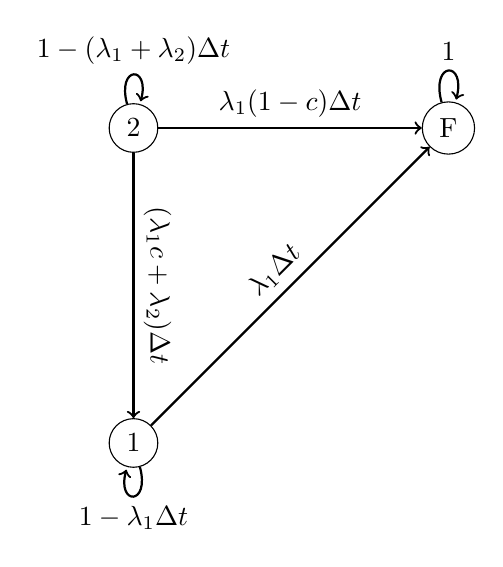
\begin{tikzpicture}
                            \tikzset{state/.style={draw, shape=circle}}
                            \node[state] (2) at (0, 4) {2};
                            \node[state] (1) at (0, 0) {1};
                            \node[state] (F) at (4, 4) {F};
                            \path[->, thick]
                                (2) edge [loop above] node {$1 - (\lambda_1 + \lambda_2)\Delta t$} (2)
                                    edge [sloped, above] node {$(\lambda_1c + \lambda_2)\Delta t$} (1)
                                    edge [above] node {$\lambda_1(1 - c)\Delta t$} (F)
                                (1) edge [loop below] node {$1 - \lambda_1\Delta t$} (1)
                                    edge [sloped, above] node {$\lambda_1\Delta t$} (F)
                                (F) edge [loop above] node {$1$} (F);
                        \end{tikzpicture}
                    \end{center}

                \item[(2)] $P(t) = \begin{bmatrix} P_2(t) \\ P_1(t) \\ P_F(t) \end{bmatrix}, P_2(t) + P_1(t) + P_F(t) = 1, P(0) = \begin{bmatrix} 1 \\ 0 \\ 0 \end{bmatrix}$

                    $A = \begin{bmatrix}
                        1 - (\lambda_1 + \lambda_2)\Delta t & 0 & 0 \\
                        (\lambda_1 c + \lambda_2)\Delta t & 1 - \lambda_1\Delta t & 0 \\
                        \lambda_1(1 - c)\Delta t & \lambda_1\Delta t & 1
                    \end{bmatrix}$

                    $P(t + \Delta t) = AP(t) = \begin{bmatrix}
                        P_2(t) - P_2(t)(\lambda_1 + \lambda_2)\Delta t\\
                        P_2(t)(\lambda_1 c + \lambda_2)\Delta t + P_1(t) - P_1(t)\lambda_1\Delta t \\
                        P_2(t)\lambda_1(1 - c)\Delta t + P_1(t)\lambda_1\Delta t + P_F(t)
                    \end{bmatrix}$

                    $\frac{P_2(t + \Delta t) - P_2(t)}{\Delta t} = P_2(t)(\lambda_1 + \lambda_2)$

                    $\frac{P_1(t + \Delta t) - P_1(t)}{\Delta t} = P_2(t)(\lambda_1 c + \lambda_2) - P_1(t)\lambda_1$

                    $\frac{P_F(t + \Delta t) - P_F(t)}{\Delta t} = P_2(t)\lambda_1(1 - c) + P_1(t)\lambda_1$

                    As $\Delta_t \to 0$, we get the differential equations for the Markov model:

                    $\frac{dP_2(t)}{dt} = P_2(t)(\lambda_1 + \lambda_2)$

                    $\frac{dP_1(t)}{dt} = P_2(t)(\lambda_1 c + \lambda_2) - P_1(t)\lambda_1$

                    $\frac{dP_F(t)}{dt} = P_2(t)\lambda_1(1 - c) + P_1(t)\lambda_1$

                    We can integrate these using the Laplace Transform:

                    $sP_2(s) - P_2(0) = sP_2(s) - 1 = -P_2(s)(\lambda_1 + \lambda_2)$

                    $P_2(s + \lambda_1 + \lambda_2) = 1 \implies P_2(s) = \frac{1}{s + \lambda_1 + \lambda_2} \implies P_2(t) = e^{-(\lambda_1 + \lambda_2)t} $

                    $sP_1(s) - P_1(0) = sP_1(s) = P_2(s)(\lambda_1c + \lambda_2) - P_1(s)\lambda_1$

                    $P_1(s)(s + \lambda_1) = P_2(s)(\lambda_1c + \lambda_2) = \frac{\lambda_1c + \lambda_2}{s + \lambda_1 + \lambda_2}$

                    $P_1(s) = \frac{\lambda_1c + \lambda_2}{(s + \lambda_1 + \lambda_2)(s + \lambda_1)} = \frac{\lambda_1c}{(s + \lambda_1 + \lambda_2)(s + \lambda_1)} + \frac{\lambda_2}{(s + \lambda_1 + \lambda_2)(s + \lambda_1)}$

                    $P_1(s) = \frac{\lambda_1c}{(s + \lambda_1 + \lambda_2)(s + \lambda_1)} + \frac{1}{s + \lambda_1} - \frac{1}{s + \lambda_1 + \lambda_2} $

            \end{description}

        \item
            \begin{enumerate}
                \item Software Implemented Fault Tolerance (SIFT) is where we use software to make systems tolerant against hardware faults. Common examples of this include implementing the voter for an NMR system in software, or using software to implement system checkpoints.

                Software Fault Tolerance (SFT) is using fault tolerance techniques for programming errors. Examples of this include acceptance tests and N-version programming.

                \item
                    \begin{description}
                        \item[(a)] The probability of a routine having no faults is $1 - 0.01 = 0.99$

                        Therefore the probrability of there being no faults in the whole program is $0.99^{20} = 0.8179$

                        \item[(b)] If the probability of the routine being faulty is reduced to $10\%$ of the original level, then the new probability is:

                        $0.01 * 0.1 = 0.001$

                        Thus the probability of a program consisting of only this routine not being faulty is $1 - 0.001 = 0.999$

                        \item[(c)] The probability of version having no faults is $0.99^{20} = 0.8179$, as stated in part \textbf{(a)}.

                        The probability of a version being faulty is the opposite of this probability: $1 - 0.99^{20} = 0.1821$

                        The probability of the whole program when three-version programming being used is therefore:

                        $(0.99^{20})^3 + 3 * (0.99^{20})^2 * (1 - 0.99^{20}) * 0.85 = 0.8577$
                    \end{description}
            \end{enumerate}

    \end{enumerate}

\end{document}
